\chapter{First Examples}
We will now look at a simple example to demonstrate the basics of how Bayesian
statistics works. We start with some probabilities at the beginning of the problem (these are
called {\it prior probabilities}), and how exactly these get updated
when we get more information (these updated probabilities are called
{\it posterior probabilities}). To help make things more clear, we will
use a table that we will call a {\it Bayes' Box} to help us calculate the
posterior probabilities easily.

Suppose there are two balls in a bag. We know in advance
that at least one of them is black, but we're not sure whether they're both
black, or whether one is black and one is white. These are the only two
possibilities we will consider.
To keep things concise, we
can label our two competing hypotheses. We could call them whatever we want,
but I will call them \bb~and \bw. So, at the beginning of the problem, we know
that {\it one and only one} of the following statements/hypotheses is true:\\
\begin{framed}
\bb: Both balls are black\\
\bw: One ball is black and the other is white.
\end{framed}
Suppose an experiment is performed to help us determine
which of these two hypotheses is
true. The experimenter reaches into the bag, pulls out one of the balls, and
observes its colour. The result of this experiment is (drumroll please!):
\begin{framed}
$D$: The ball that was removed from the bag was black.
\end{framed}
We will now do a Bayesian analysis of this result.

\section{The Bayes' Box}
A Bayesian analysis starts by choosing some values for the prior probabilities.
We have our two competing hypotheses \bb~and \bw, and we need to choose some
probability values to describe how sure we are that each of these is true.
Since we are talking about two hypotheses, there will be two prior probabilities,
one for \bb~and one for \bw.
For simplicity, we will assume that we don't have much of an idea which is true,
and so we will use the following prior probabilities:
\begin{eqnarray}
P(\bb) &=& 0.5\\
P(\bw) &=& 0.5.
\end{eqnarray}
Pay attention to the notation. The upper case $P$ stands for probability, and if we just
write $P(\texttt{whatever})$, that means we are talking about the
prior probability of {\tt whatever}. We will see the notation for the posterior probability
shortly. Note also that since the two hypotheses are mutually exclusive
(they can't both be true) and exhaustive (one of these is true, it can't be
some undefined third option).
We will almost always consider mutually exclusive and exhaustive hypotheses in
this course\footnote{If this does not appear to be true in a particular problem,
it is usually possible to redefine the various hypotheses into a set that of
hypotheses that {\it are}
mutually exclusive and exhaustive.}.

The choice of 0.5 for the two prior probabilities describes the fact that,
before we did the experiment, we were very uncertain about which of the two
hypotheses was true.
I will now present a {\it Bayes' Box}, which lists all the hypotheses (in this
case
two) that might be true, and the prior probabilities. There are some extra
columns which we haven't discussed yet, and will be needed in order to
figure out the posterior probabilities in the final column.
\begin{table}[!ht]
\begin{center}
\begin{tabular}{|c|c|c|c|c|}
\hline
{\bf Hypotheses} & {\tt prior} & {\tt likelihood} &
{\tt prior $\times$ likelihood} & {\tt posterior}\\
\hline
\bb & 0.5 &   &  & \\
\bw & 0.5 &   &  & \\
\hline
Totals: & 1 & & & \\
\hline
\end{tabular}
\end{center}
\end{table}
The first column of a Bayes' Box is just the list of hypotheses we are
considering. In this case there are just two. If you need to construct a Bayes' box for a new problem, just think
about what the possible answers to the problem are, and list them in the first
column. The second column lists the prior probabilities for each of the
hypotheses.
Above, before we did the experiment, we decided to say that there was a 50\%
probability that \bb~is true and a 50\% probability that \bw~is true, hence the 0.5 values in this column.
The prior column should always sum to 1. Remember, the prior probabilities
only describe our initial uncertainty, before taking the data into account. Hopefully the data will help by changing these probabilities to
something a bit more decisive.

\subsection{Likelihood}
The third column is called {\it likelihood}, and this is a really important
column where the action happens. The likelihood is a quantity
that will be used for calculating the posterior
probabilities.
In colloquial language, likelihood is synonymous with
probability. It means the same thing. However, in statistics, likelihood is a
very
specific kind of probability. To fill in the third column of the Bayes' Box,
we need to calculate two likelihoods, so you can tell from this that the
likelihood is something different for each hypothesis. But what is it
exactly?
\begin{framed}
{\bf The likelihood for a hypothesis is the probability that you would have
observed the data, if that hypothesis were true. The values can be found by
going through each hypothesis in turn, imagining it is true, and asking,
``What is the probability of getting the data that I observed?''.}
\end{framed}

Here is the Bayes' Box with the likelihood column filled in. I will explain
how these numbers were calculated in a bit more detail in the next subsection.
\begin{table}[!ht]
\begin{center}
\begin{tabular}{|c|c|c|c|c|}
\hline
{\bf Hypotheses} & {\tt prior} & {\tt likelihood} &
{\tt h = prior $\times$ likelihood} & {\tt posterior}\\
\hline
{\tt BB} & 0.5 & 1 &  & \\
{\tt BW} & 0.5 & 0.5 &  & \\
\hline
Totals: & 1 & & & \\
\hline
\end{tabular}
\end{center}
\end{table}
If you have taken STATS 210 and used the maximum likelihood method, where you
find the value of a parameter that maximises the likelihood function, that is
the same as the likelihood we use in this course! So you have a head start
in understanding this concept.

\subsection{Finding the Likelihood Values}
We will first calculate the value of the likelihood for the \bb~hypothesis.
Remember, the data we are analysing here is that we chose one of the balls in
the bag ``at random'', and it was black. The likelihood for the \bb~hypothesis is
therefore the probability that we would get a black ball if \bb~is true.

Imagine that \bb~is true. That means both balls are black. What is the probability that
the experiment would result in a black ball? That's easy -- it's 100\%! So we
put the number 1 in the Bayes Box as the likelihood for the \bb~hypothesis.

Now imagine instead that \bw~is true. That would mean one ball is black and the
other is white. If this were the case and we did the experiment, what would be
the probability of getting the black ball in the experiment? Since one of the
two balls is black, the chance of choosing this one is 50\%. Therefore, the
likelihood for the \bw~hypothesis is 0.5, and that's why I put 0.5 in the Bayes'
Box for the likelihood for \bw.

In general, the likelihood is the {\it probability of the data that you actually
got, assuming a particular hypothesis is true}. In this example it was
fairly easy to get the likelihoods directly by asking ``if this hypothesis
is true, what is the probability of getting the black ball when we do the
experiment?''. Sometimes this is not so easy, and it can be helpful to think about
ALL possible experimental outcomes/data you might have seen -- even though
ultimately, you just need to select the one that actually occurred.
Table~\ref{tab:all_data} shows an example of this process.

\begin{table}[!ht]
\begin{center}
\begin{tabular}{|c|c|c|}
\hline
{\bf Hypotheses} & {\bf Possible Data} & {\bf Probability} \\
\hline
{\tt BB} & {\color{blue} Black Ball} & {\color{blue} 1}\\
         & White Ball & 0 \\
\hline
{\tt BW} & {\color{blue} Black Ball} & {\color{blue} 0.5} \\
         & White Ball & 0.5 \\
\hline
\end{tabular}
\caption{\it This table demonstrates a method for calculating the likelihood
values, by considering not just the data that actually occurred, but all
data that might have occurred. Ultimately, it is only the probability of the
data which actually occurred that matters, so this is highlighted in blue.
\label{tab:all_data}}
\end{center}
\end{table}
The fact that only the blue probabilities in Table~\ref{tab:all_data} enter the
Bayes' Box calculation is related to the {\it likelihood principle}, which we
will
discuss in lectures. Note also that in Table~\ref{tab:all_data}, the
probabilities for the different possible data sets add to 1 within each
hypothesis, but the sum of the blue ``selected'' likelihood values is not 1
(it is, in fact, meaningless).

When we come to parameter estimation in later chapters, we will usually set up
our problems in this way, by considering what data sets are possible, and
assigning probabilities to them.

\subsection{The Mechanical Part}
The third column of the Bayes' Box is the product of the prior probabilities
and the likelihoods, calculated by simple multiplication. The result will be
called ``prior times likelihood'', but occasionally we will use the letter $h$
for these quantities. This is the {\it unnormalised} posterior. It does not sum
to 1 as the posterior probabilities should, but it is at least proportional to
the actual posterior probabilities.

To find the posterior probabilities, we take the {\tt prior $\times$ likelihood}
column and divide it by its sum, producing numbers that do sum to 1. This
gives us the final
posterior probabilities, which were the goal all along. The completed Bayes'
Box is shown below:

\begin{table}[!ht]
\begin{center}
\begin{tabular}{|c|c|c|c|c|}
\hline
{\bf Hypotheses} & {\tt prior} & {\tt likelihood} &
{\tt h = prior $\times$ likelihood} & {\tt posterior}\\
\hline
{\tt BB} & 0.5 & 1 & 0.5 & 0.667\\
{\tt BW} & 0.5 & 0.5 & 0.25  & 0.333\\
\hline
Totals: & 1 & & 0.75 & 1\\
\hline
\end{tabular}
\end{center}
\end{table}
We can see that the posterior probabilities are not the same as the prior
probabilities, because we have more information now! The experimental result
made \bb~a little bit more plausible than it was before. Its probability has
increased from 1/2 to 2/3.

\subsection{Interpretation}
The posterior probabilities of the hypotheses are proportional to the prior probabilies
and the likelihoods. A high prior probability will help a hypothesis have a high
posterior probability. A high likelihood value also helps.
To understand what this means about reasoning, consider
the meanings of the prior and the likelihood. There are two things that can
contribute to a hypothesis being plausible:
\begin{itemize}
\item If the prior probability is high. That is, the hypothesis was {\it already}
plausible, before we got the data.
\item If the hypothesis {\it predicted the data} well. That is, the data was
what we would have expected to occur if the hypothesis had been true.
\end{itemize}
I hope you agree that this is all very sensible.

In class we will also study
variations on this problem, considering different assumptions about the prior
probabilities and how they affect the results, and also considering what happens
when we get more and/or different data.

\section{Bayes' Rule}
Bayes' rule is an equation from probability theory, shown in
Figure~\ref{fig:bayes_neon}. The various terms in Bayes' rule are all
probabilities, but notice that there are conditional probabilities in there.
For example, the left hand side of the equation is $P(A|B)$ and that means
the probability of $A$ {\bf given} $B$. That is, it's the probability of $A$
after taking into account the information $B$. In other words,
$P(A|B)$ is a posterior probability, and Bayes' rule tells us how to calculate
it from other probabilities.
\begin{figure}[!ht]
\begin{center}
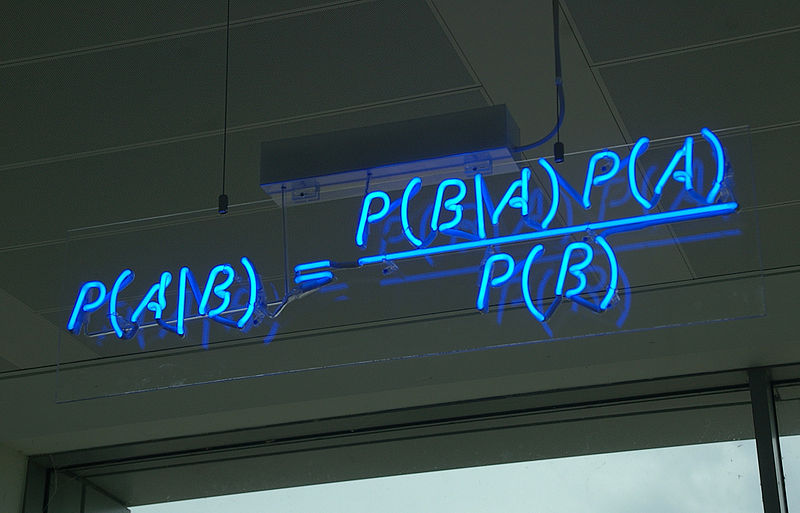
\includegraphics[scale=0.4]{Figures/bayes_neon.jpg}
\caption{\it A blue neon sign displaying Bayes' rule.
You can use it to calculate the probability of $A$ {\it given} $B$,
if you know the values of some other probabilities on the right hand side.
Image credit: Matt Buck. Obtained from Wikimedia Commons.
\label{fig:bayes_neon}}
\end{center}
\end{figure}
Bayes' rule is true for {\it any} statements $A$ and $B$. If you took the
equation in Figure~\ref{fig:bayes_neon} and replaced $A$ with
``K\={a}k\={a}p\={o} will survive beyond 2050'' and $B$ with
``I had coffee this morning'', the
resulting equation would still be true\footnote{It would still be true, but
it would not very interesting,
because
whether or not I had coffee doesn't tell you much about the survival prospects
of endangered New Zealand parrots.}.

It is helpful to relabel $A$ and $B$ in Bayes' rule to give a more clear
interpretation of how the equation is to be used. In this version of Bayes'
rule (which is one you should commit to memory), $A$ has been replaced by $H$,
and $B$ has been replaced by $D$. The reason for these letters is that you should
interpret $H$ as {\it hypothesis} and $D$ as {\it data}. Then you can interpret
Bayes' rule as telling you the probability of a hypothesis given some data, in
other words, a posterior probability.
\begin{eqnarray}
P(H|D) = \frac{P(H)P(D|H)}{P(D)}
\end{eqnarray}
In Bayesian statistics, most of the terms in Bayes' rule have special names.
Some of them even have more than one name, with different scientific
communities preferring different terminology. Here is a list of the
various terms and the names we will use for them:
\begin{itemize}
\item $P(H|D)$ is the {\bf posterior probability}. It describes how certain
or confident we are that
hypothesis $H$ is true, given that we have observed data $D$. Calculating
posterior probabilities is the main goal of Bayesian statistics!
\item $P(H)$ is the {\bf prior probability}, which describes how sure we were
that $H$ was true, before we observed the data $D$.
\item $P(D|H)$ is the {\bf likelihood}. If you were to assume that $H$ is true,
this is the probability that you would have observed data $D$.
\item $P(D)$ is the {\bf marginal likelihood}. This is the probability that you
would have observed data $D$, {\it whether $H$ is true or not}.
\end{itemize}
Since you may encounter Bayesian methods outside of STATS 331, I have included
an Appendix called ``Rosetta Stone'' that lists some common alternative
terminology.

In the above example, we did some calculations to work out the numbers in the
Bayes' Box, particularly the posterior probabilities, which are the ultimate
goal of the calculation. {\it What we were actually doing in these calculations
was applying Bayes' rule}. We actually applied Bayes' rule twice, once to
compute $P(\bb | D)$ and a second time to calculate $P(\bw | D)$.

\begin{framed}
{\bf When you use a Bayes' Box to calculate posterior probabilities,
you are really just applying Bayes' rule a lot of times:
once for each hypothesis listed in the first column.}
\end{framed}

\section{Phone Example}
This example is based on Question 1 from the 2012 final exam. I got the
idea for this question from an example in David MacKay's wonderful book
``Information Theory, Inference and Learning Algorithms''
(available online as a free PDF download. You're welcome to check it out, but
it is a large book and only about 20\% of the content is relevant to this course!).

You move into a new house which has a phone
installed. You can't remember the phone number, but you suspect it
might be {\tt 555-3226} (some of you may recognise
this as being the phone number for Homer Simpson's ``Mr Plow'' business).
To test this hypothesis, you carry out an experiment
by picking up the phone and dialing {\tt 555-3226}.

If you are correct about
the phone number, you will definitely hear a busy signal because you are calling
yourself.
If you are incorrect, the probability of hearing a busy signal is $1/100$.
However, all of that is only true if you assume the phone is working, and it
might be broken! If the phone is broken, it will always give a busy signal.

When you do the experiment, the outcome (the data) is that you do actually get the busy signal.
The question asked us to consider the following four hypotheses, and to calculate
their posterior probabilities:
\begin{table}[!ht]
\begin{center}
\begin{tabular}{|c|c|c|c|}
\hline
Hypothesis & Description & Prior Probability\\
\hline
$H_1$ & Phone is working and {\tt 555-3226} is correct & 0.4\\
$H_2$ & Phone is working and {\tt 555-3226} is incorrect & 0.4\\
$H_3$ & Phone is broken and {\tt 555-3226} is correct & 0.1\\
$H_4$ & Phone is broken and {\tt 555-3226} is incorrect & 0.1\\
\hline
\end{tabular}
\caption{\it The four hypotheses about the state of the phone and the phone
number. The prior probabilities are also given.
\label{tab:phone}}
\end{center}
\end{table}
Note that the four hypotheses are mutually exclusive and exhaustive. If you were
to come up with hypotheses yourself, ``phone is working'' and ``{\tt 555-3226} is correct''
might spring to mind. They wouldn't be mutually exclusive so you couldn't do a
Bayes' Box with just those two, but it is possible to put these together (using
``{\bf and}'') to make the four mutually exclusive options in the table.

\subsection{Solution}
We will go through the solution using a Bayes' Box. The four hypotheses listed
in Table~\ref{tab:phone} and their prior probabilities are given, so we can fill
out the first two columns of a Bayes' Box right away:
\begin{table}[!ht]
\begin{center}
\begin{tabular}{|c|c|c|c|c|}
\hline
{\bf Hypotheses} & {\tt prior} & {\tt likelihood} &
{\tt prior $\times$ likelihood} & {\tt posterior}\\
\hline
$H_1$ & 0.4 &  &  & \\
$H_2$ & 0.4 &  &  & \\
$H_3$ & 0.1 &  &  & \\
$H_4$ & 0.1 &  &  & \\
\hline
Totals: & 1 & & & \\
\hline
\end{tabular}
\end{center}
\end{table}
The next thing we need is the likelihoods. The outcome of the experiment (the
data) was the busy signal, so we need to work out $P(\textnormal{busy signal} | H)$ for each $H$
in the problem (there are four of them). Let's start (naturally!) with $H_1$.

If we assume $H_1$ is true, then the phone is working and {\tt 555-3226} is the
correct phone number. In that case, we would definitely get a busy signal
because we are calling ourselves. Therefore
$P(\textnormal{busy signal} | H_1) = 1$ is our first likelihood value.

Next, let's imagine that $H_2$ is true, so the phone is working, but
{\tt 555-3226} is not the right phone number. In this case, it is given in the
question that the probability of getting a busy signal is $1/100$ or 0.01 (in
reality, this would be based on some other data, or perhaps be a totally
subjective judgement).
Therefore $P(\textnormal{busy signal} | H_2) = 0.01$, and that's our second
likelihood value.

The likelihoods for $H_3$ and $H_4$ are quite straightforward
because they both imply the phone is broken, and that means a busy signal is certain.
Therefore $P(\textnormal{busy signal} | H_3) = P(\textnormal{busy signal} | H_4) = 1$.
We have our four likelihoods, and can proceed to work out everything in the
Bayes' Box, including the main goal -- the posterior probabilities! Here it is:
\begin{table}[!ht]
\begin{center}
\begin{tabular}{|c|c|c|c|c|}
\hline
{\bf Hypotheses} & {\tt prior} & {\tt likelihood} &
{\tt prior $\times$ likelihood} & {\tt posterior}\\
\hline
$H_1$ & 0.4 & 1 &  0.4 & 0.662\\
$H_2$ & 0.4 & 0.01 & 0.004 & 0.00662\\
$H_3$ & 0.1 & 1 & 0.1 & 0.166\\
$H_4$ & 0.1 & 1 & 0.1 & 0.166\\
\hline
Totals: & 1 & & 0.604 & 1\\
\hline
\end{tabular}
\end{center}
\end{table}

To conclude this phone problem, I should admit that
I actually calculated the numbers in the Bayes' Box using R. My code is shown
below. A lot of the code we write in labs will look like this. Obviously in the
2012 exam the students had to use their calculators instead.
\begin{minted}[mathescape,
               numbersep=5pt,
               gobble=0,
               frame=single,
               framesep=2mm, fontsize=\small]{r}
prior = c(0.4, 0.4, 0.1, 0.1) # Vector of prior probs
lik = c(1, 0.01, 1, 1)        # Vector of likelihoods
h = prior*lik
Z = sum(h)                    # Sum of prior times likelihood
post = prior*lik/Z            # Normalise to get posterior
# Look at all the results
print(prior)
print(lik)
print(h)
print(Z)
print(post)
\end{minted}

Now let's try to see if this makes sense. There are many things we could think
about, but let's just consider the question of whether
the phone is working or not. The first two hypotheses correspond to the phone
being in a working state. If you want to calculate the probability of $A$
{\bf or} $B$, then you can just add the probabilities if they are mutually
exclusive. The prior probability that the phone is working is
therefore:
\begin{eqnarray}
P(\textnormal{phone working}) &=& P(H_1 \textbf{ or } H_2)\\
&=& P(H_1) + P(H_2)\\
&=& 0.4 + 0.4\\
&=& 0.8.
\end{eqnarray}
The posterior probability is worked out in a similar way, but using the posterior
probabilities instead of the prior ones:
\begin{eqnarray}
P(\textnormal{phone working}|\textnormal{busy signal}) &=& P(H_1 \textbf{ or } H_2 | \textnormal{busy signal})\\
&=& P(H_1|\textnormal{busy signal}) + P(H_2|\textnormal{busy signal})\\
&=& 0.662 + 0.00662\\
&=& 0.6689.
\end{eqnarray}
Our probability that the phone is working has gone down a little bit as a result of this
evidence! That makes sense to me. A busy signal is what you would expect to
happen if the phone was broken. This data doesn't {\it prove} the phone is
broken, but it does point in that direction a little bit, and hence the
probability that the phone is working has been reduced from 0.8 to 0.6689.

\section{Important Equations}
Posterior probabilities are calculated using Bayes' rule. For a single
hypothesis $H$ given data $D$, Bayes' rule is:
\begin{eqnarray}
P(H|D) = \frac{P(H)P(D|H)}{P(D)}\label{eq:bayes1}
\end{eqnarray}
This gives the posterior probability $P(H|D)$ in terms of the prior probability
$P(H)$, the likelihood $P(D|H)$ and the marginal likelihood $P(D)$ in the
denominator. To obtain $P(H)$, think about your prior beliefs (which may
indicate a large amount of uncertainty, or may already be well informed based
on previous data sets). To obtain $P(D|H)$, think about what the experiment is
doing: If $H$ is true, what data would you expect to see and with what
probabilities?

The denominator is the probability of obtaining the data $D$ but without
assuming that $H$ is either true or false. This is obtained using the sum rule.
There are two ways that the data $D$ could occur, either via the route of $H$
being true (this has probability $P(H)P(D|H)$), or via the route of $H$ being
false (this has probability $P(\bar{H})P(D|\bar{H})$). These two ways are
mutually exclusive, so we can add their probabilities:
\begin{eqnarray}
P(D) = P(H)P(D|H) + P(\bar{H})P(D|\bar{H}).
\end{eqnarray}

Bayes' rule can be applied to a whole set
of hypotheses (that are mutually exclusive and exhaustive) simultaneously.
This is a more common way of using it, and it is the way we use it when we use
a Bayes' Box. If we applied Equation~\ref{eq:bayes1} to $N$ hypotheses
$H_1, H_2, ..., H_N$, given data $D$, we would get the following for the posterior
probability of each hypothesis $H_i$ (for $i=1, 2, ..., N$):
\begin{eqnarray}
P(H_i|D) &=& \frac{P(H_i)P(D|H_i)}{P(D)}
\end{eqnarray}
The denominator $P(D)$ is a single number. It does not depend on the index $i$.
It can again be obtained using the sum rule. There are $N$
mutually exclusive ways that the data $D$ could have occurred: via $H_1$ being
true, or via $H_2$ being true, etc. Adding the probabilities of these gives:
\begin{eqnarray}
P(D) &=& \sum_{i=1}^N P(H_i)P(D|H_i).
\end{eqnarray}
which just happens to be the sum of the prior times likelihood values.
If you don't find equations particularly easy to read, just remember that
following the steps for making a Bayes' Box is equivalent to applying
Bayes' rule in this form! The $P(H_i)$ values are the prior probability column, the
$P(D|H_i)$ values are the likelihood column, and the denominator is the
sum of the prior times likelihood column. For example, the posterior probability
for $H_1$ (the top right entry in a Bayes' Box) is given by the prior probability
for $H_1$ times the likelihood for $H_1$, divided by the sum of prior times
likelihood values. That is, $P(H_1|D) = P(H_1)P(D|H_1)/P(D)$.
The correspondence between the probabilities that go in a Bayes'
Box (in general) and the terms in the Equations are given in
Table~\ref{tab:general_bayes_box}.

\begin{table}[!ht]
\begin{center}
\begin{tabular}{|c|c|c|c|c|}
\hline
{\bf Hypotheses} & {\tt prior} & {\tt likelihood} &
{\tt prior $\times$ likelihood} & {\tt posterior}\\
\hline
$H_1$ & $P(H_1)$ & $P(D|H_1)$ & $P(H_1)\times P(D|H_1)$ & $P(H_1|D)$\\
$H_2$ & $P(H_2)$ & $P(D|H_2)$ & $P(H_2)\times P(D|H_2)$ & $P(H_2|D)$\\
\ldots & \ldots & \ldots & \ldots & \ldots\\
\hline
Totals: & 1 & & $P(D)$ & 1\\
\hline
\end{tabular}
\caption{\it A general Bayes' Box. Using Bayes' rule or making a Bayes' Box are
actually the same thing, and this table can be used to identify the
terms.\label{tab:general_bayes_box}}
\end{center}
\end{table}

